
%(BEGIN_QUESTION)
% Copyright 2010, Tony R. Kuphaldt, released under the Creative Commons Attribution License (v 1.0)
% This means you may do almost anything with this work of mine, so long as you give me proper credit

Contractors install this vortex flowmeter, equipped with a pulse output (1 pulse per 25 gallons), to totalize flow through a pipe:

$$\includegraphics[width=15.5cm]{i00053x01.eps}$$

Unfortunately, the flow computer connected to this circuit is not registering any accumulated flow, even though an operator has verified flow through the pipe at approximately 370 gallons per minute.  Your first step is to disconnect the flow computer input from this circuit (so it is wired exactly as shown) then to take your DC voltmeter and measure voltage between terminals 1 and 4: there, your meter registers 23.1 volts DC.  Your next step is to measure DC voltage across the collector and emitter terminals of the optocoupler's transistor: there your meter registers 0 volts.

Identify the likelihood of each specified fault for this circuit.  Consider each fault one at a time (i.e. no coincidental faults), determining whether or not each fault could independently account for {\it all} measurements and symptoms in this circuit.

% No blank lines allowed between lines of an \halign structure!
% I use comments (%) instead, so that TeX doesn't choke.

$$\vbox{\offinterlineskip
\halign{\strut
\vrule \quad\hfil # \ \hfil & 
\vrule \quad\hfil # \ \hfil & 
\vrule \quad\hfil # \ \hfil \vrule \cr
\noalign{\hrule}
%
% First row
{\bf Fault} & {\bf Possible} & {\bf Impossible} \cr
%
\noalign{\hrule}
%
% Another row
$R_1$ failed open &  &  \cr
%
\noalign{\hrule}
%
% Another row
$R_2$ failed open &  &  \cr
%
\noalign{\hrule}
%
% Another row
$R_1$ failed shorted &  &  \cr
%
\noalign{\hrule}
%
% Another row
$R_2$ failed shorted &  &  \cr
%
\noalign{\hrule}
%
% Another row
1 amp fuse blown &  &  \cr
%
\noalign{\hrule}
%
% Another row
100 milliamp fuse blown &  &  \cr
%
\noalign{\hrule}
%
% Another row
24 VDC source dead &  &  \cr
%
\noalign{\hrule}
%
% Another row
5 VDC source dead &  &  \cr
%
\noalign{\hrule}
} % End of \halign 
}$$ % End of \vbox

Finally, identify the {\it next} diagnostic test or measurement you would make on this system.  Explain how the result(s) of this next test or measurement help further identify the location and/or nature of the fault.

\vfil

\underbar{file i00053}
\eject
%(END_QUESTION)





%(BEGIN_ANSWER)


%(END_ANSWER)





%(BEGIN_NOTES)

% No blank lines allowed between lines of an \halign structure!
% I use comments (%) instead, so that TeX doesn't choke.

$$\vbox{\offinterlineskip
\halign{\strut
\vrule \quad\hfil # \ \hfil & 
\vrule \quad\hfil # \ \hfil & 
\vrule \quad\hfil # \ \hfil \vrule \cr
\noalign{\hrule}
%
% First row
{\bf Fault} & {\bf Possible} & {\bf Impossible} \cr
%
\noalign{\hrule}
%
% Another row
$R_1$ failed open &  & $\surd$ \cr
%
\noalign{\hrule}
%
% Another row
$R_2$ failed open & $\surd$ &  \cr
%
\noalign{\hrule}
%
% Another row
$R_1$ failed shorted &  & $\surd$ \cr
%
\noalign{\hrule}
%
% Another row
$R_2$ failed shorted & $\surd$ &  \cr
%
\noalign{\hrule}
%
% Another row
1 amp fuse blown &  & $\surd$ \cr
%
\noalign{\hrule}
%
% Another row
100 milliamp fuse blown & $\surd$ &  \cr
%
\noalign{\hrule}
%
% Another row
24 VCDC source dead &  & $\surd$ \cr
%
\noalign{\hrule}
%
% Another row
5 VCDC source dead & $\surd$ &  \cr
%
\noalign{\hrule}
} % End of \halign 
}$$ % End of \vbox

If $R_2$ were failed shorted, it would blow the 100 mA fuse at the next pulse, thereby creating a 0 volt drop across the optocoupler's C-E terminals.






\filbreak \vskip 20pt \vbox{\hrule \hbox{\strut \vrule{} {\bf Virtual Troubleshooting} \vrule} \hrule}

\noindent
{\bf Predicting the effect of a given fault:} present each of the following faults to the students, one at a time, having them comment on all the effects each fault would produce.

\begin{itemize}
\item{} 
\item{} 
\item{} 
\end{itemize}


\vskip 10pt


\noindent
{\bf Identifying possible/impossible faults:} present symptoms to the students and then have them determine whether or not a series of suggested faults could account for all the symptoms, explaining {\it why} or {\it why not} for each proposed fault:

\begin{itemize}
\item{} Symptom: {\it }
\item{}  -- {\bf Yes/No}
\item{}  -- {\bf Yes/No}
\item{}  -- {\bf Yes/No}
\end{itemize}


\vskip 10pt


\noindent
{\bf Determining the utility of given diagnostic tests:} present symptoms to the students and then propose the following diagnostic tests one by one.  Students rate the value of each test, determining whether or not it would give useful information (i.e. tell us something we don't already know).  Students determine what different results for each test would indicate about the fault, if anything:

\begin{itemize}
\item{} Symptom: {\it The flow computer receives a 5 volt DC signal all the time, regardless of flow}
\item{} Measure voltage between terminals 1 and 3 -- {\bf Yes}
\item{} Measure voltage between terminals 5 and 8 -- {\bf No}
\item{} Check 1 amp fuse -- {\bf No}
\item{} Measure voltage between terminals 7 and 8 -- {\bf Yes}
\item{} Measure resistance between terminals 9 and 11 -- {\bf Yes}
\item{} Check 100 milliamp fuse -- {\bf No}
\item{} Measure 5 volt power supply output with voltmeter -- {\bf No}
\item{} Measure voltage between terminals 5 and 7 -- {\bf Yes}
\item{} Measure 24 volt power supply output with voltmeter -- {\bf No}
\end{itemize}


\vskip 10pt


\noindent
{\bf Diagnosing a fault based on given symptoms:} imagine the ??? fails ??? in this system (don't reveal the fault to students!).  Present the operator's observation(s) to the students, have them consider possible faults and diagnostic strategies, and then tell them the results of tests they propose based on the following symptoms, until they have properly identified the nature and location of the fault:

\begin{itemize}
\item{} Operator observation: {\it }
\item{} 
\item{} 
\end{itemize}
%INDEX% Measurement, flow: vortex flow element
%INDEX% Troubleshooting review: electric circuits

%(END_NOTES)


